\documentclass[tikz]{standalone}
\usepackage{tikz}
\usetikzlibrary{graphs, shapes.geometric}
\usepackage{tkz-graph}

\begin{document}
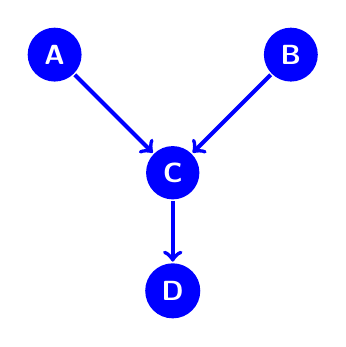
\begin{tikzpicture}
    \SetVertexNormal[Shape = circle,
                 FillColor = orange,
                 LineWidth = 2pt]
    \SetUpEdge[lw = 1.5pt,
        color = blue]
    \SetGraphUnit{3}
    \tikzset{vertex/.style={font = \sffamily\bfseries,
                text = white,shape = circle,
                fill = blue,
                very thick}}
    \node[vertex] (A) at (3.5,3) {A};
    \node[vertex] (B) at (6.5,3) {B};
    \node[vertex] (C) at (5,1.5) {C};
    \node[vertex] (D) at (5,0) {D};
    \tikzset{EdgeStyle/.style={->}}
    \Edge(B)(C)
    \Edge(C)(D)
    \Edge(A)(C)
\end{tikzpicture}
\end{document}